% !TeX program = pdflatex
% =============================================================
% Public Economics -- Lecture 11
% State and Local Government Expenditure
% Based on: Gruber, J. "Public Finance and Public Policy", Ch. 10
% =============================================================
\documentclass[11pt,aspectratio=169]{beamer}

\usetheme{metropolis}
\usepackage[utf8]{inputenc}
\usepackage[T1]{fontenc}
\usepackage{lmodern}
\usepackage{booktabs}
\usepackage{array}
\usepackage{textcomp}
\usepackage{siunitx}
\usepackage{tikz}
\usepackage{pgfplots}
\pgfplotsset{compat=1.18}
\usetikzlibrary{positioning,arrows.meta,calc}

% ----------------------------------------------------------------
% Colors: WU Vienna blue as primary accent
% ----------------------------------------------------------------
\definecolor{wublue}{HTML}{003D7C}
\definecolor{wulight}{HTML}{4F8FC4}
\definecolor{wugray}{HTML}{5C6670}
\definecolor{wured}{HTML}{B0202E}
\definecolor{wugreen}{HTML}{4C8C6B}
\definecolor{wuyellow}{HTML}{D9A441}
\setbeamercolor{palette primary}{bg=wublue,fg=white}
\setbeamercolor{frametitle}{bg=wublue,fg=white}
\setbeamercolor{progress bar}{fg=wublue,bg=wulight!30}
\setbeamercolor{alerted text}{fg=wured}

\setbeamertemplate{frame footer}{State \& Local Government}
\setbeamertemplate{footline}[frame number]

\title{Public Economics}
\subtitle{Lecture 11 \(\cdot\) State and Local Government Expenditure}
\author{Shushanik Margaryan}
\institute{WU Vienna University of Economics and Business}
\date{Winter Term}

% Source note command for footnote-style citations on data slides
\newcommand{\srcnote}[1]{{\footnotesize\color{wugray}Source: #1}}

\begin{document}

% =============================================================
\begin{frame}
  \titlepage
\end{frame}

\begin{frame}{Today's Questions}
  \begin{itemize}
    \item Which public goods should be provided \emph{nationally}, and which are better left to states, regions, or municipalities?
    \item Can people ``vote with their feet'' by choosing where to live --- and does that solve the preference-revelation problem that plagues national public-goods provision?
    \item Why do higher levels of government so often send money down to lower ones, and does that money get spent the way we'd expect?
  \end{itemize}
  \vspace{1em}
  \begin{block}{Based on}
    Gruber, J. \emph{Public Finance and Public Policy}, Ch.\ 10 (State and Local Government Expenditures).
  \end{block}
\end{frame}

% =============================================================
\begin{frame}{Outline}
  \tableofcontents
\end{frame}

% =============================================================
\section{10.1 Fiscal Federalism}

\begin{frame}{Why Multiple Levels of Government?}
  Almost every country splits public provision across national, regional, and local governments. Two forces pull in opposite directions:
  \begin{itemize}
    \item \textbf{Centralization} lets government exploit \textbf{economies of scale} and internalize \textbf{spillovers} across jurisdictions (national defense benefits everyone; a local government has no incentive to pay for it alone).
    \item \textbf{Decentralization} lets provision match \textbf{local tastes}, which vary --- a beach town and a mountain town may want very different mixes of public services.
  \end{itemize}
\end{frame}

\begin{frame}{The Decentralization Theorem}
  \begin{block}{Oates's decentralization theorem (1972)}
    When preferences for a public good vary across localities, and there are no spillovers or scale economies, welfare is higher under \textbf{decentralized}, locally tailored provision than under a single uniform national level of provision.
  \end{block}
  \vspace{0.4em}
  \small Intuition: a single national quantity necessarily overshoots some areas' preferences and undershoots others'. Local governments can each choose the level their own residents actually want.
\end{frame}

\begin{frame}{Optimal Fiscal Federalism: What Goes Where?}
  The efficient assignment of a public good to a level of government depends on two things: the \textbf{size of spillovers} across jurisdictions, and the \textbf{degree of taste heterogeneity}.
  \begin{center}
  \small
  \begin{tabular}{@{}lp{3.6cm}p{3.3cm}@{}}
    \toprule
    & \textbf{Large spillovers / scale economies} & \textbf{Local tastes vary a lot} \\
    \midrule
    National defense & \checkmark & \\
    Environmental regulation & \checkmark & \\
    Local parks, trash collection & & \checkmark \\
    Local zoning, policing style & & \checkmark \\
    \bottomrule
  \end{tabular}
  \end{center}
  \vspace{0.3em}
  \small Goods with large spillovers or scale economies belong at the national level; goods with strong local taste variation and few spillovers belong at the local level. Most real public goods sit somewhere in between.
\end{frame}

% =============================================================
\section{10.2 The Tiebout Model}

\begin{frame}{Tiebout (1956): ``Voting with Your Feet''}
  National elections force everyone to accept the \emph{same} bundle of public goods and taxes --- one vote cannot reveal how much any individual actually values it.
  \begin{block}{Tiebout's insight}
    If there are \textbf{many local communities}, each offering a different bundle of local public goods and local taxes, people can simply \textbf{move} to the community that best matches their preferences.
  \end{block}
  \vspace{0.4em}
  \small This ``voting with your feet'' behaves like a market: it reveals preferences (through location choice) in a way that a single national vote never can --- potentially solving the preference-revelation problem central to public-goods theory.
\end{frame}

\begin{frame}{The Origin Story: Shopping and Competition}
  \small
  Tiebout's 1956 question: what does the \emph{private} market have that guarantees efficient provision, which the market for public goods lacks? His answer: \textbf{shopping and competition}.
  \begin{itemize}
    \item If a firm sells an inferior product, customers buy from a competitor instead --- that threat of exit disciplines private firms.
    \item Voters can ``shop'' across national candidates too, but a vote for Congress or President bundles together hundreds of issues, and changing policy is slow --- weak discipline.
  \end{itemize}
  \begin{alertblock}{A vivid contrast}
    Learning the US Department of Defense paid \$437 for a tape measure (1980s) gives you no real recourse --- you won't emigrate over it. But learning your \emph{local library} paid \$37,000 for its director's sports car (New York City, 2014) gives you a real option: \textbf{move to the town next door.}
  \end{alertblock}
\end{frame}

\begin{frame}{The Tiebout Model: Assumptions}
  The result is elegant, but relies on strong assumptions:
  \begin{enumerate}
    \setlength{\itemsep}{2pt}
    \item Many communities exist, each already offering a distinct tax/service bundle.
    \item Individuals are \textbf{perfectly mobile} and can move costlessly.
    \item Full information about every community's taxes and services.
    \item No spillovers between communities.
    \item At least as many communities as there are distinct sets of tastes.
    \item Communities can adjust to their \textbf{optimal size} (not too crowded, not too empty).
    \item No economies of scale in providing local public goods.
  \end{enumerate}
\end{frame}

\begin{frame}{The Formal Model}
  Many individuals sort themselves across towns. Town $i$ has $N_i$ residents and finances spending $G_i$ with a \textbf{uniform tax} of $G_i/N_i$ on every resident.
  \begin{block}{Tiebout's result}
    In equilibrium, individuals sort themselves so that everyone within a given town shares the \textbf{same} taste for public goods --- and so demands the same $G_i$.
  \end{block}
  \small This solves \emph{both} problems that plague national public-goods provision:
  \begin{itemize}
    \item \textbf{No revelation problem:} with a uniform tax and identical neighbors, nobody has anything to gain by lying about their preferences.
    \item \textbf{No aggregation problem:} the town government just divides its residents' shared preferred spending level by the population.
  \end{itemize}
\end{frame}

\begin{frame}{Worked Example: Jack, Ava, and Tiebout}
  Recall Jack and Ava from the Lindahl-pricing example (Lecture 9): fireworks cost 75\textcent\ each.
  \begin{itemize}
    \item Jack joins a town of 100 people just like him. They vote for \textbf{75} fireworks, each paying 56\textcent.
    \item Suppose Jack tries his old trick: claiming Ava's (lower) preferences. In the Tiebout model, he can't just \emph{say} it --- he has to \textbf{act} on it, by moving to a town of people like Ava, who only want \textbf{25} fireworks, at 19\textcent\ each.
  \end{itemize}
  \begin{alertblock}{No more free-riding}
    By moving, Jack pays a third as much --- but gets only a third as many fireworks. He has \emph{no incentive} to lie, because lying means actually living with the consequences. Lindahl pricing, which failed nationally, works automatically once people sort into like-minded towns.
  \end{alertblock}
\end{frame}

\begin{frame}{Diagram: Sorting Across Communities}
  \begin{center}
  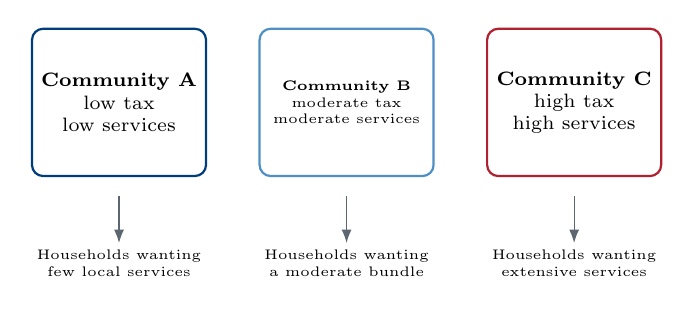
\begin{tikzpicture}[scale=0.85]
    \draw[wublue, thick, rounded corners] (0,0) rectangle (2.6,2.2);
    \node[align=center, font=\scriptsize] at (1.3,1.1) {\textbf{Community A}\\ low tax\\ low services};
    \draw[wulight, thick, rounded corners] (3.4,0) rectangle (6.0,2.2);
    \node[align=center, font=\tiny] at (4.7,1.1) {\textbf{Community B}\\ moderate tax\\ moderate services};
    \draw[wured, thick, rounded corners] (6.8,0) rectangle (9.4,2.2);
    \node[align=center, font=\scriptsize] at (8.1,1.1) {\textbf{Community C}\\ high tax\\ high services};
    \draw[-{Latex}, wugray] (1.3,-0.3) -- (1.3,-1.0);
    \draw[-{Latex}, wugray] (4.7,-0.3) -- (4.7,-1.0);
    \draw[-{Latex}, wugray] (8.1,-0.3) -- (8.1,-1.0);
    \node[align=center, font=\tiny] at (1.3,-1.3) {Households wanting\\ few local services};
    \node[align=center, font=\tiny] at (4.7,-1.3) {Households wanting\\ a moderate bundle};
    \node[align=center, font=\tiny] at (8.1,-1.3) {Households wanting\\ extensive services};
  \end{tikzpicture}
  \end{center}
  \footnotesize Each household self-selects into the community whose tax/service bundle matches its own preferences --- mimicking, through residential choice, the preference revelation an ordinary market provides for private goods.
\end{frame}

\begin{frame}{Problems with Tiebout Competition}
  \small
  \begin{itemize}
    \setlength{\itemsep}{3pt}
    \item \textbf{Imperfect mobility:} moving means leaving your job, friends, and community behind --- most people are far more ``stuck'' than the model assumes.
    \item \textbf{Imperfect information:} you'd likely never learn your library was buying its director sports cars unless local media happened to expose it.
    \item \textbf{Limited range of substitute towns:} the model needs \emph{many} nearby towns to choose from --- true in dense suburbs (e.g., around Boston), far less true in smaller or more spread-out metro areas.
    \item \textbf{The scale tension:} Tiebout needs \emph{enough towns} for people to sort into like-minded groups, but also needs each town to be \emph{large enough} to fund public goods (schools, parks) efficiently. These two requirements pull in opposite directions.
  \end{itemize}
\end{frame}

\begin{frame}{Problems with Tiebout Financing: Lump-Sum Taxes}
  The formal model requires financing public goods with a \textbf{lump-sum tax} --- a fixed amount, identical for every resident, regardless of income.
  \begin{itemize}
    \item Widely seen as deeply \textbf{inequitable}: rich and poor residents pay exactly the same amount.
    \item As a result, lump-sum taxes are almost never actually used to fund government.
  \end{itemize}
  \begin{alertblock}{The Thatcher poll tax (1990)}
    The UK's most prominent attempt at a lump-sum local tax --- replacing local property taxes with a flat per-resident ``community charge'' --- triggered major riots and led directly to the resignation of an otherwise enormously popular prime minister.
  \end{alertblock}
\end{frame}

\begin{frame}{The Property-Tax Free-Rider Problem --- and Zoning}
  In practice, towns finance public goods with a \textbf{property tax} proportional to home value --- which creates a new problem.
  \begin{itemize}
    \item Since richer neighbors pay more in absolute tax dollars for the \emph{same} local services, everyone has an incentive to live in a town with people \textbf{richer than themselves} --- free-riding on their neighbors' tax payments.
  \end{itemize}
  \begin{block}{Zoning}
    Restrictions towns place on the use of real estate --- setbacks, bans on running a business from home, minimum lot sizes, and bans on multifamily housing.
  \end{block}
  \small Zoning protects a town's tax base by pricing lower-income households out of the housing market. Glaeser \& Gyourko (2002) find that land in zoned areas costs roughly \textbf{10 times} as much as comparable land in unzoned markets.
\end{frame}

\begin{frame}{No Externalities/Spillovers}
  The model assumes a town's public goods affect \emph{only} that town --- rarely true.
  \begin{itemize}
    \item \textbf{A new park:} enjoyed mostly by your town, but visited by neighbors too --- since your town only weighs its \emph{own} residents' benefit, the park gets \textbf{underprovided} relative to the social optimum.
    \item \textbf{Police:} an under-resourced department can push crime into neighboring towns.
    \item \textbf{Public works:} potholed streets slow down through-traffic from elsewhere too.
    \item \textbf{Education:} a more educated citizenry benefits the whole country, not just the town that paid for the schooling.
  \end{itemize}
  \small The fundamental trade-off: local provision suits small, like-minded towns well, but goods with real spillovers are better handled --- or subsidized via grants --- at a higher level of government.
\end{frame}

\begin{frame}{Evidence: Resident Similarity Across Communities}
  \begin{block}{Testable prediction}
    The \emph{more} communities there are to choose from, the more residents can sort into like-minded towns --- so tastes for public goods should be \textbf{more similar within towns} where choice is greater.
  \end{block}
  \small \textbf{Gramlich \& Rubinfeld (1982):} surveying Michigan households, preferences for public goods were more similar within towns in larger metro areas (more towns to choose from) than in smaller areas --- and satisfaction with public spending was correspondingly higher.\\
  \textbf{Bergstrom et al.\ (1986):} using the same Michigan data, found that local public-goods provision satisfied the efficiency condition that marginal cost equals the \emph{sum} of residents' marginal rates of substitution --- direct support for the model.
\end{frame}

\begin{frame}{Evidence: Tax and Service Capitalization}
  If the Tiebout logic holds, a community's fiscal bundle should show up directly in \textbf{local property values} --- people ``vote with their pocketbook,'' not just their feet.
  \begin{block}{Capitalization}
    A locality's fiscal bundle (taxes net of the services they fund) becomes built into the price of housing there.
  \end{block}
  \small Oates (1969) finds exactly this: holding housing characteristics constant, property values are higher where local school spending is higher, and lower where local property tax rates are higher.\\
  \srcnote{Oates (1969), \emph{JPE} 77(6).}
\end{frame}

\begin{frame}{Evidence: Capitalization and California's Proposition 13}
  \textbf{Rosen (1982)} studies Prop 13 (1978), which capped California property tax rates at 1\% of assessed value --- a sharp, quasi-experimental cut concentrated in previously high-tax towns.
  \begin{itemize}
    \item Comparing $\sim$60 San Francisco-area towns before/after the vote: each \textbf{\$1} of property-tax reduction raised house values by about \textbf{\$7}.
    \item At $\sim$12\% interest rates, \emph{full} capitalization would predict $1/0.12 \approx \$8.33$ per dollar --- so \$7 implies capitalization close to complete.
  \end{itemize}
  \small This is a large effect: it implies Californians didn't expect to lose much in local services from the tax cut. That optimism wasn't entirely borne out --- prosperous San Jose had to cut art and music teachers, nurses, and library hours, and its school district became the first in 40 years to declare bankruptcy (1983).\\
  \srcnote{Rosen (1982), \emph{Journal of Political Economy}.}
\end{frame}

\begin{frame}{Evidence: Are We Under-Investing in Local Public Goods?}
  \small
  \textbf{Cellini, Ferreira \& Rothstein (2010):} a regression-discontinuity design comparing school districts where a capital-spending bond \emph{barely} passed to those where it \emph{barely} failed. Where it passed, home values rose substantially --- buyers would pay \textbf{\$1.50 or more} for every \$1 of capital spending.
  \vspace{0.3em}

  \textbf{Bayer et al.\ (2020):} compare districts more vs.\ less affected by court orders mandating increased spending in the \emph{lowest}-spending school districts. House prices rose more where mandated spending increases were largest --- and the implied benefit of extra (especially teacher-salary) spending exceeds the tax cost by more than the resulting tax increases reduce house prices.
  \begin{alertblock}{Implication}
    Nationally, we may be systematically \textbf{under-spending} on tax-financed education relative to what residents would actually value.
  \end{alertblock}
\end{frame}

\begin{frame}{Optimal Fiscal Federalism: Three Factors}
  \small
  Even though the Tiebout model is unrealistic taken literally, it tells us what \emph{should} guide the assignment of public goods to levels of government:
  \begin{enumerate}
    \setlength{\itemsep}{3pt}
    \item \textbf{Tax-benefit linkages:} how directly residents see their taxes tied to what they get back. Strong linkage (local roads: your property tax buys better roads for you) $\Rightarrow$ provide locally. Weak linkage (welfare: most residents don't benefit from redistribution to the poor) $\Rightarrow$ provide at the state/federal level, since taxpayers will otherwise ``vote with their feet'' away from generous towns.
    \item \textbf{Spillovers:} goods with large spillovers (or without any private substitute) are underprovided locally --- push these up to where the government can internalize the full benefit, or add grants.
    \item \textbf{Economies of scale:} goods with large scale economies (national defense) aren't efficiently produced by many small, competing localities; goods without them (police, garbage collection) are well suited to local Tiebout competition.
  \end{enumerate}
\end{frame}

\begin{frame}{Does US Fiscal Federalism Match the Theory?}
  \small Broadly, yes:
  \begin{itemize}
    \item \textbf{Public works} (roads, garbage, street cleaning): strong tax-benefit linkage, few spillovers, low scale economies --- financed \textbf{locally}, as predicted.
    \item \textbf{Redistribution} (cash welfare): weak tax-benefit linkage --- financed at the \textbf{state and federal} level, as predicted.
    \item \textbf{National defense}: enormous scale economies --- a purely \textbf{national} program, as predicted.
    \item \textbf{Education}: real spillovers (a better-educated citizenry benefits the whole country) --- financed roughly \textbf{half locally, half by higher government} (mostly state). The open question: the federal government provides under 10\% of education funding, far less than in most other industrialized nations --- are education's nationwide spillovers large enough to justify a bigger federal role?
  \end{itemize}
\end{frame}

\begin{frame}{Application: Regulatory Federalism}
  The same logic extends beyond spending to \textbf{regulation}: narrowly local issues should be regulated locally; issues with spillovers, redistributive stakes, or scale economies belong at a higher level.
  \begin{itemize}
    \item States have recently taken a much more aggressive role in \textbf{overriding} local regulations --- on the minimum wage, gun control, smoking bans, and transgender bathroom policies.
    \item Some of these have plausible spillover logic (a locality with looser gun laws may effectively supply weapons to stricter neighbors); others (bathroom policies) have no obvious spillover at all.
  \end{itemize}
  \small Grabar (2016) and Badger (2017) suggest that the rising political \textbf{polarization} discussed in the Political Economy lecture may itself be pushing state-local regulatory conflict away from what Tiebout-style efficiency principles would recommend.
\end{frame}

% =============================================================
\section{10.3 Redistribution and Fiscal Federalism}

\begin{frame}{The Problem with Local Redistribution}
  If Tiebout sorting works well for allocating \emph{public goods}, it works badly for \textbf{redistribution}.
  \begin{alertblock}{The race to the bottom}
    A generous local welfare program attracts low-income residents and repels high-income taxpayers who would have to fund it --- eroding the local tax base and forcing benefits back down. Anticipating this, no locality wants to be the first mover, and redistribution ends up systematically \textbf{under-provided} at the local level.
  \end{alertblock}
  \small This is a standard argument for financing redistributive programs at the \textbf{national}, not local, level --- where the tax base can't simply relocate to a neighboring town.
\end{frame}

\begin{frame}{Tax Competition Among Jurisdictions}
  The same mobility logic applies to \textbf{capital and corporate taxation}, not just welfare recipients.
  \begin{itemize}
    \item Firms and mobile capital can relocate toward jurisdictions offering lower tax rates.
    \item Jurisdictions competing for this mobile tax base face pressure to cut rates below what they would otherwise choose --- a fiscal ``race to the bottom'' on the tax-collection side.
  \end{itemize}
  \small As with local redistribution, this is an argument for coordinating certain tax bases (especially highly mobile ones like corporate income) above the purely local level.
\end{frame}

\begin{frame}{Fiscal Disparities Across Jurisdictions}
  Communities differ enormously in their underlying \textbf{tax base} --- a wealthy suburb can fund excellent local schools at a low tax rate; a poor rural district cannot fund comparable schools even at a much higher rate.
  \begin{itemize}
    \item Left alone, Tiebout sorting reinforces this: the wealthy cluster together, the poor cluster together, and local service quality diverges further.
    \item This is the standard efficiency-\emph{and}-equity case for \textbf{intergovernmental grants}: transfers from higher levels of government to lower ones, to offset unequal local tax capacity.
  \end{itemize}
\end{frame}

% =============================================================
\section{10.4 Intergovernmental Grants}

\begin{frame}{Types of Grants: Categorical vs.\ Block}
  \begin{itemize}
    \item \textbf{Categorical (matching) grant:} the higher government matches every dollar the local government spends on a specific service (e.g., \$1 in federal money for every \$2 in local road spending). This \textbf{lowers the effective price} of that service to the locality.
    \item \textbf{Block (non-matching) grant:} a fixed lump sum, with no strings attached to how it's spent (or only broad strings, e.g., ``for education''). This acts like a pure \textbf{increase in local income}.
  \end{itemize}
  \small The distinction matters enormously for how local governments actually respond --- a price effect versus an income effect.
\end{frame}

\begin{frame}{Diagram: Matching Grants vs.\ Block Grants}
  \begin{columns}[T]
    \begin{column}{0.56\textwidth}
      \begin{tikzpicture}[scale=0.36]
        \draw[-{Latex}] (0,0) -- (13,0) node[below, font=\scriptsize]{Public good $G$};
        \draw[-{Latex}] (0,0) -- (0,10.5) node[left, font=\scriptsize]{Private good $C$};
        \draw[wugray, thick] (0,6) -- (6,0);
        \draw[wugreen, thick, dashed] (0,9) -- (9,0);
        \draw[wured, thick] (0,6) -- (12,0);
      \end{tikzpicture}
    \end{column}
    \begin{column}{0.44\textwidth}
      \scriptsize
      \textcolor{wugray}{\textbf{Gray:}} original budget line.\\[0.3em]
      \textcolor{wugreen}{\textbf{Green:}} block grant --- parallel shift, a pure income effect.\\[0.3em]
      \textcolor{wured}{\textbf{Red:}} matching grant --- pivots from the same intercept, lowers the price of $G$.
    \end{column}
  \end{columns}
  \vspace{0.3em}
  \scriptsize A matching grant induces more spending on $G$ per dollar of grant than an equal-sized block grant, since it changes a relative price, not just income.
\end{frame}

\begin{frame}{The Flypaper Effect}
  Standard theory predicts that a \$1,000 lump-sum grant to a local government should raise local public spending by roughly the same small amount that a \$1,000 increase in \emph{residents' own income} would --- both are just income effects of the same size.
  \begin{alertblock}{The flypaper effect}
    Empirically, this prediction fails badly: a grant paid directly to the local government raises local spending by far \textbf{more} than an equivalent rise in residents' private income does. ``Money sticks where it hits.''
  \end{alertblock}
  \small Leading explanations include imperfect information (residents don't realize the grant could instead be passed back as a tax cut), and the incentives of local bureaucrats and officials who directly control the grant funds and prefer to spend rather than rebate them.
\end{frame}

\begin{frame}{Conclusion}
  \begin{itemize}
    \item Fiscal federalism trades off the scale/spillover advantages of centralization against the taste-matching advantages of decentralization.
    \item The Tiebout model shows how residential mobility \emph{can} solve the preference-revelation problem for local public goods --- but only under demanding assumptions that rarely hold exactly.
    \item Redistribution and highly mobile tax bases are the clearest case \emph{against} full decentralization --- and intergovernmental grants are the standard tool for correcting the resulting fiscal disparities, even though how localities actually respond to grants (the flypaper effect) doesn't always match the textbook prediction.
  \end{itemize}
\end{frame}

% =============================================================
\begin{frame}{Sources}
  \tiny
  \begin{columns}[T]
    \begin{column}{0.5\textwidth}
      Gruber, J., \emph{Public Finance and Public Policy}, Ch.\ 10.\\
      Oates, W. (1969), \emph{JPE} 77(6).
    \end{column}
    \begin{column}{0.5\textwidth}
      Oates, W. (1972), \emph{Fiscal Federalism}.\\
      Tiebout, C. (1956), \emph{JPE} 64(5).
    \end{column}
  \end{columns}
\end{frame}

\begin{frame}[standout]
  Thank you!\\
  \vspace{0.5em}
  \small Questions and discussion
\end{frame}

\end{document}
